\chapter{Data Assimilation}
\chaptermark{DA} %this is the chapter heading that will show on subsequent pages

Specifically, I test a MATLAB implentation of the Extended Kalman Filter (EKF) and Ensemble Kalman Filter (EnKF) on the Lorenz 1963 three-variable model:
\begin{align*}
\frac{dx}{dt} &= \sigma (y-x)\\
\frac{dy}{dt} &= rx - y -xz \\
\frac{dz}{dt} &= xy -  bz\end{align*}

The cannonical choice of $\sigma = 10, b = 8/3$ and $r = 28$ is used for all tests here, which produce the well known butterfly attractor (Figure \ref{fig:lorenzattractor}).

\subsection{3D-Var}

Most operational weather centers today operate with a 3D-var filter.

\subsection{Extended Kalman Filter}

For starters, I coded an EKF.
The EKF is the ``gold standard'' of data assimilation methods.
It works by updating our knowledge of error covariance matrix for each assimilation window, using a Tangent Linear Model (TLM).
Using the notation of Kalnay \cite{kalnay2003}, this amounts to making a forecast with the nonlinear model $M$, and updating the error covariance matrix $P$ with the TLM $L$, and adjoint model $L^T$

\begin{align*} x^f (t_i) &= M _{i-1} [x ^a (t_{i-1} ) ]\\
P^f (t_i ) &= L_{i-1} P^a (t_{i-1} ) L^T _{i-1} + Q (t_{i-1} ) \end{align*}

where $Q$ is the noise covariance matrix (model error).
Here $Q = 0$ since our model is perfect.

The analysis step is then written as (for $H$ the observation operator):

\begin{align*} x^a (t_i ) &= x^f (t_i) + K_i d_i\\
P^a (t_i) &= (I - K_i H_i )P^f (t_i) \end{align*}

where
\[ d_i = y_i^o - H[x^f (t_i) ] \]
is the innovation.

The Kalman gain matrix is computed to minimize the analysis error covariance $P^a _i$ as
\[ K_i = P^f (t_i) H_i ^T [ R_i + H_i P^f (t_i) H^T ] ^{-1} \]
where $R_i$ is the observation error covariance.

Since we are making observations of the truth with random normal errors of standard deviation $\epsilon$, then $R_i$ is a matrix of just $\epsilon$ values.

The most difficult, and most computationally expensive, part of the EKF is deriving and integrating the TLM.
For this reason, no operational weather centers use the EKF, although approximations such as the EnKF are promising (next).

\subsection{Ensemble Kalman Filter}

The computational cost of the EKF is mitigated through the approximation of the error covariance matrix $C_f$ from an ensemble of predictions.

As an alternative to the prohibitively costly EKF, filters which approximate the error covariance matrix from other methods are gaining wind.
One such approach is the use of a forecast ensemble, where a collection of models (ensemble members) are initialized from the prior analysis $x^a$ with random error.
The spread of these models with randoms errors is then used to estimate the error covariance.

\begin{figure}[tpb!]
  \centering
  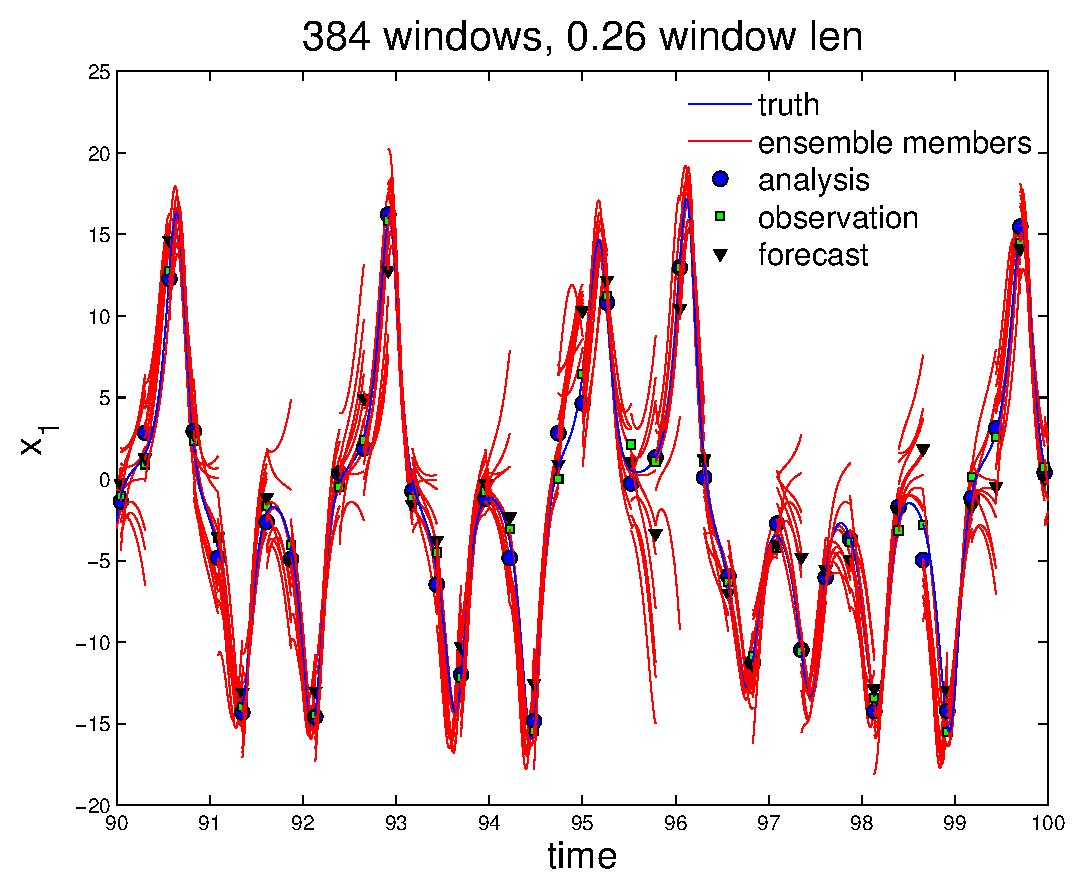
\includegraphics[width=0.49\textwidth]{figures/EnKF_spaghetti.pdf}
  \caption{
    A sample timeseries of the ensembles used in the EnKF.
    In all tests, as seen here, 10 ensemble members are used.
  }
  \label{fig:spaghetti}
\end{figure}

\begin{figure}[tpb!]
  \centering
  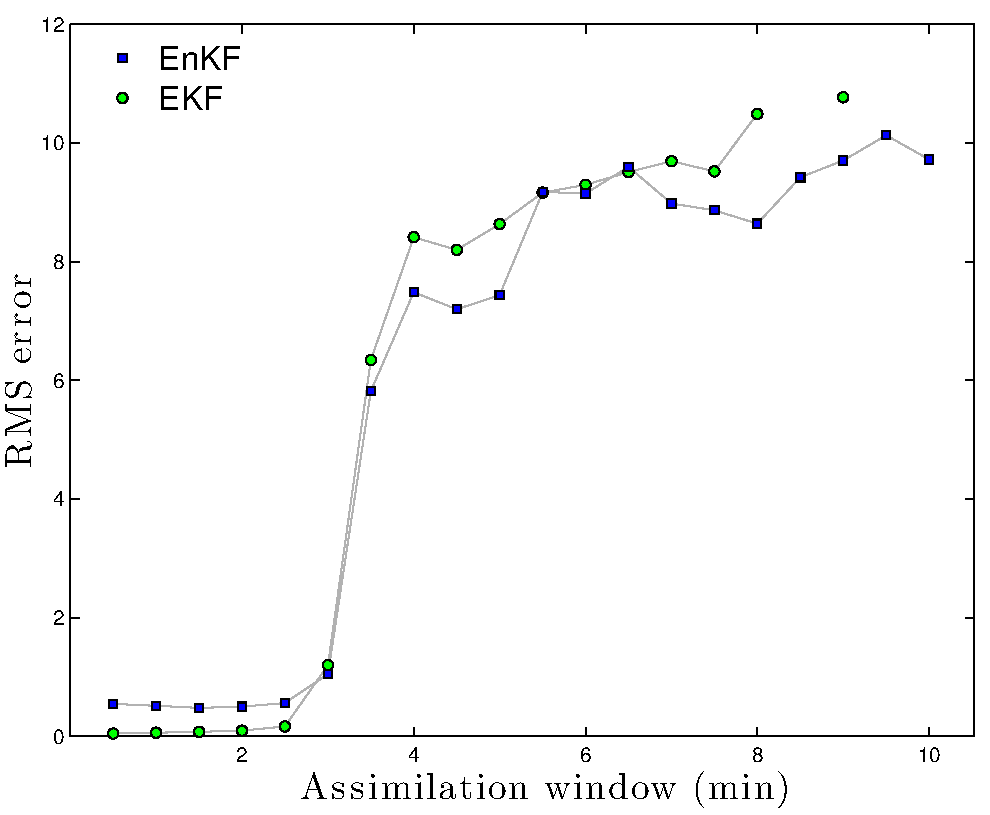
\includegraphics[width=0.49\textwidth]{figures/window_experiment_plot001.pdf}
  \caption{
    The RMS error (unscaled by climatology) is reported for our EKF and EnKF filters, measured as the difference between forecast and truth at the end of an assimiliation window for the latter 2500 assimiliation windows in a 3000 assimilation window model run.
    Error is measured in the only observed variable, $x_1$.
    Increasing the assimilation window led to an decrease in predictive skill, as expected.
    Additive and multiplicative covariance inflation is the same as Harris et. al., I've ran a few experiments to tune these, I should have my own tuning for every window length soon.    
  }
  \label{fig:window_test}
\end{figure}

\begin{figure}[tpb!]
  \centering
  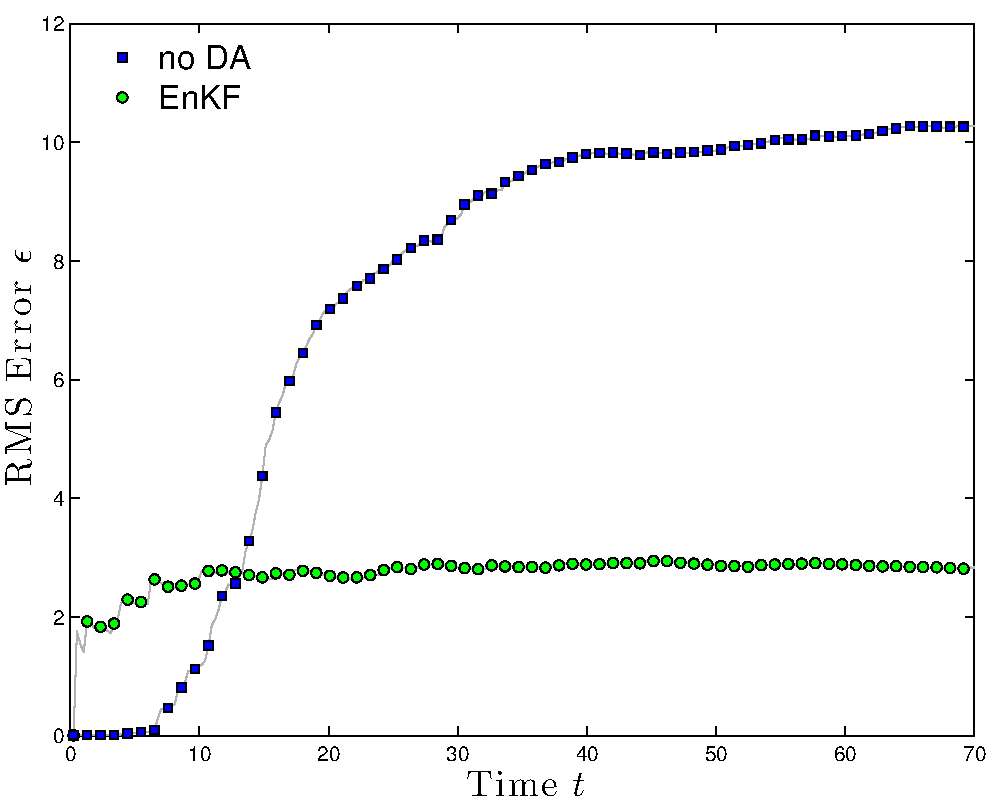
\includegraphics[width=0.49\textwidth]{figures/DA_test_noname2.pdf}
  \caption{
    For near-perfect initial knowledge of the atmospheric state, the RMS error of a prediction using DA is compared against a prediction that does not.
    Initial error is normal with mean 0 and variance 0.01, and the RMS errors reported are averages of 100 runs.
    Observational noise is normally distributed with mean 0 and variance 0.5, and an assimilation window length of 0.261 is used (approximately 5\% of climatological variation).
    As would be expected, in the long run DA greatly improves forecast skill, as forecasts without DA saturate to climatological error.
    The initial period where a forecast exceeds the skill of DA is potentially due to the spin-up time required by the filter to dial in the analysis error covariance.
  }
  \label{fig:DA_test}
\end{figure}

Since this method is only an approximation, it often fails to capture the full spread of error, and so additive and multiplicative inflation factors are used to obtain a good estimate of the error covariance.

The only difference between this approach and the EKF, numerically, is that the forecast error covariance $P^f$ is computed from the ensemble members, without the need for a tangent linear model:
\[ P^f \approx \frac{1}{K-2} \sum _{k\neq l} \left ( x_k ^f - \overline{x} ^f _l \right ) \left ( x_k ^f - \overline{x} ^f _l \right ) ^T .\]

\begin{figure}[tpb!]
  \centering
  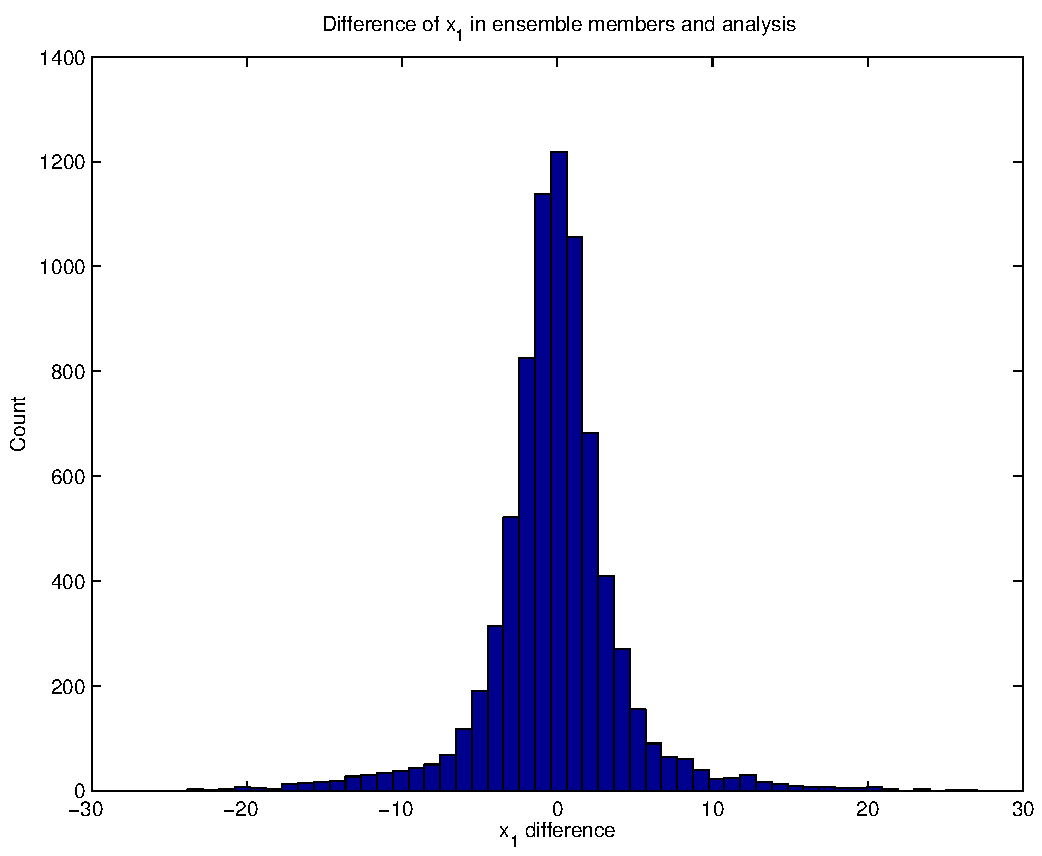
\includegraphics[width=0.49\textwidth]{figures/EnKF-histogram-analysis.pdf}
  \caption{
    The difference of ensemble forecasts from the analysis is reported for 760 assimilation windows in one model run of length 200, with 10 ensemble members and an assimilation window of length 0.261.
    This has the same shape of as the difference between enseble forecasts and the mean of the forecasts (I have this as well).
    This spread of ensemble forecasts is what allows us to estimate the error covariance of the forecast model, and appears fall from a normal distribution.
  }
  \label{fig:EnKFhist}
\end{figure}



In computing the error covariance $P$ from the ensemble, we wish to add up the error covariance of each forecast with respect to the mean forecast. 
But this would underestimate the error covariance since the forecast we're comparing was used in the ensemble average (to obtain the mean forecast).
So here to computing the error covariance matrix for each forecast, that forecast itself is excluded from the ensemble average forecast.

We can see the classic spaghetti of the ensemble with this filter implemented on Lorenz 63 in Figure \ref{fig:spaghetti}.

\section{Coding the TLM}

Actually coding the TLM was difficult, so I'll try to spell it out here, to make sure I understand it.
The TLM is the model which advances an initial perturbation $\delta x_{i}$ at timestep $i$ to a final perturbation $\delta ^* x_{i+1}$ at timestep $i+1$.
The dynamical system we are interested in, Lorenz '63, is given as a system of ODE's:
\[ \frac{dx}{dt} = F(x) .\]
We integrate this system using a numerical scheme of our choice (here I used RK2), to obtain a model $M$ discretized in time.
\[ x(t) = M[ x(t_0) ] .\]
Introducing a small perturbation $y$, we can approximate the our model $M$ of $x(t_0) + y(t_0)$ with a Taylor series around $x(t_0)$, for which we assume to already have solved for:
\begin{align*} M[ x(t_0) + y(t_0) ] &= M [ x(t_0) ] + \frac{\partial M}{\partial x} y(t_0) + O [ y(t_0) ^2 ]\\ &\approx x(t) + \frac{\partial M}{\partial x} y(t_0) .\end{align*}
We can then solve for the linear evolution of the small perturbation $y(t_0)$ as 
\[ \frac{dy }{dt } = J y \] where $J = \partial F / \partial x$ is the Jacobian of $F$.
We can solve the above system of linear ordinary differential equations using the same numerical scheme as we did for the nonlinear model.

\begin{figure}[tpb!]
  \centering
  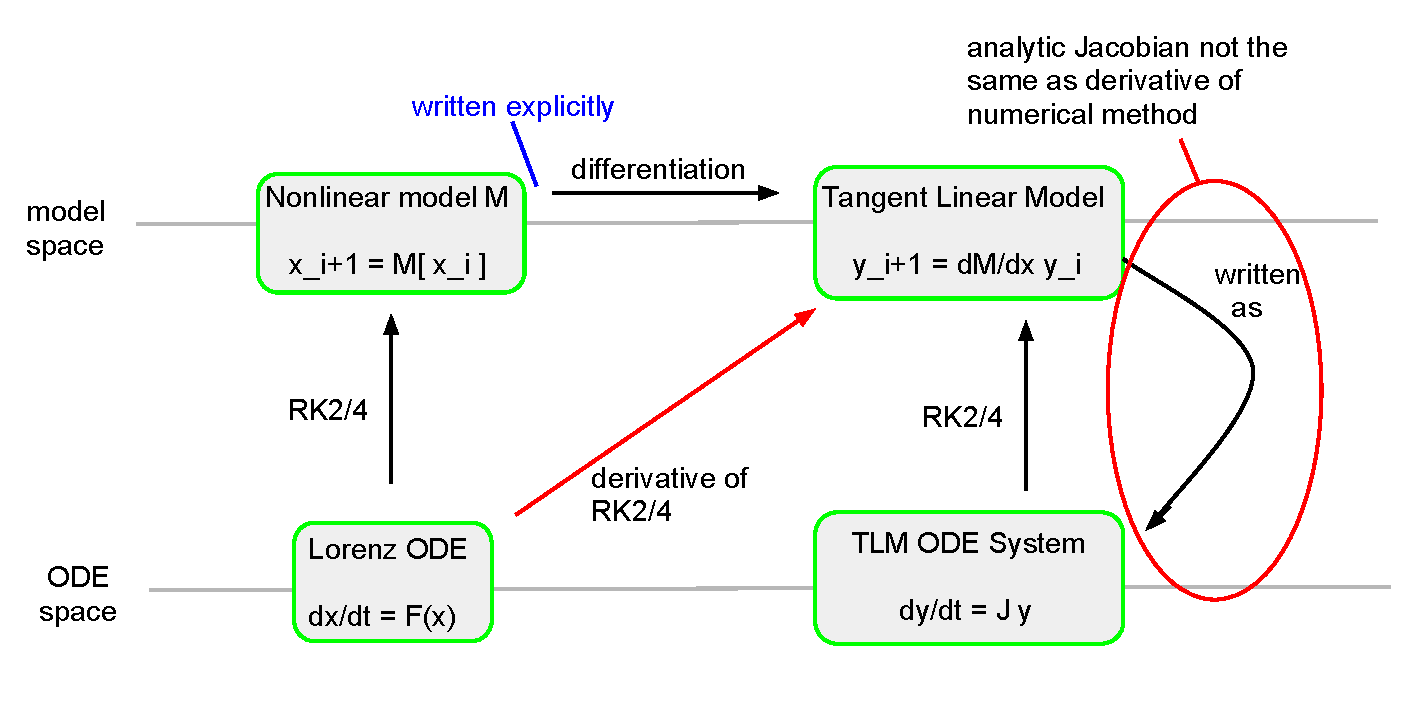
\includegraphics[width=0.49\textwidth]{figures/TLM-explanation.pdf}
  \caption{
    An explanation of how and why the best way to obtain a TLM is with a differentiated numerical scheme.
  }
  \label{fig:TLMscheme}
\end{figure}

The problem with solving that system of equations is that the Jacobian matrix of discretized code is not necessarily identical to the discretization of the Jacobian operator for the analytic system.
This is a problem because we need to have the TLM of our model $M$, which is the time-space discretization of the solution to $dx/dt = F(x)$.
We can apply our numerical method to the $dx/dt = F(x)$ to obtain $M$ explicitly, and then take the Jacobian of this.
But, that is extremely messy (and costly), since recall the RK4 method had many nested function iterations.
It is therefore desirable to take the derivative of the numerical scheme directly, and apply this differentiated numerical scheme to the system of equations $F(x)$ to obtain the TLM.
A schematic of this scenario is illustrated in Figure \ref{fig:TLMscheme}.
It is for this reason that there exists code that takes the derivative of numerical code (i.e. Fortran) for implementing the EKF on models larger than 3 dimensions with numerical schemes more complicated than RK2 or RK4.


\begin{table}[h]\caption{Summary of Lorenz '63 parameters}
\begin{center}
\begin{tabular}{|c|c|c|}
\hline
Parameter & Value & Interpretation, if any\\
\hline
$\sigma$ & 10 & \\
\hline
$b$ & 8/3 & \\
\hline
$r$ & 28 & \\
\hline
\end{tabular}
\end{center}
\end{table}

The cannonical choice of $\sigma = 10, b = 8/3$ and $r = 28$ is used for all tests here, which produce the well known butterfly attractor (Figure \ref{fig:lorenzattractor}).


